\chapter{SUPPLEMENTAL MATERIAL FOR CHAPTER VI}

\section{Supplemental Figures}
This section includes the supplemental figures and tables referenced in chapter VI.


\begin{figure}%figure S1
\centering
	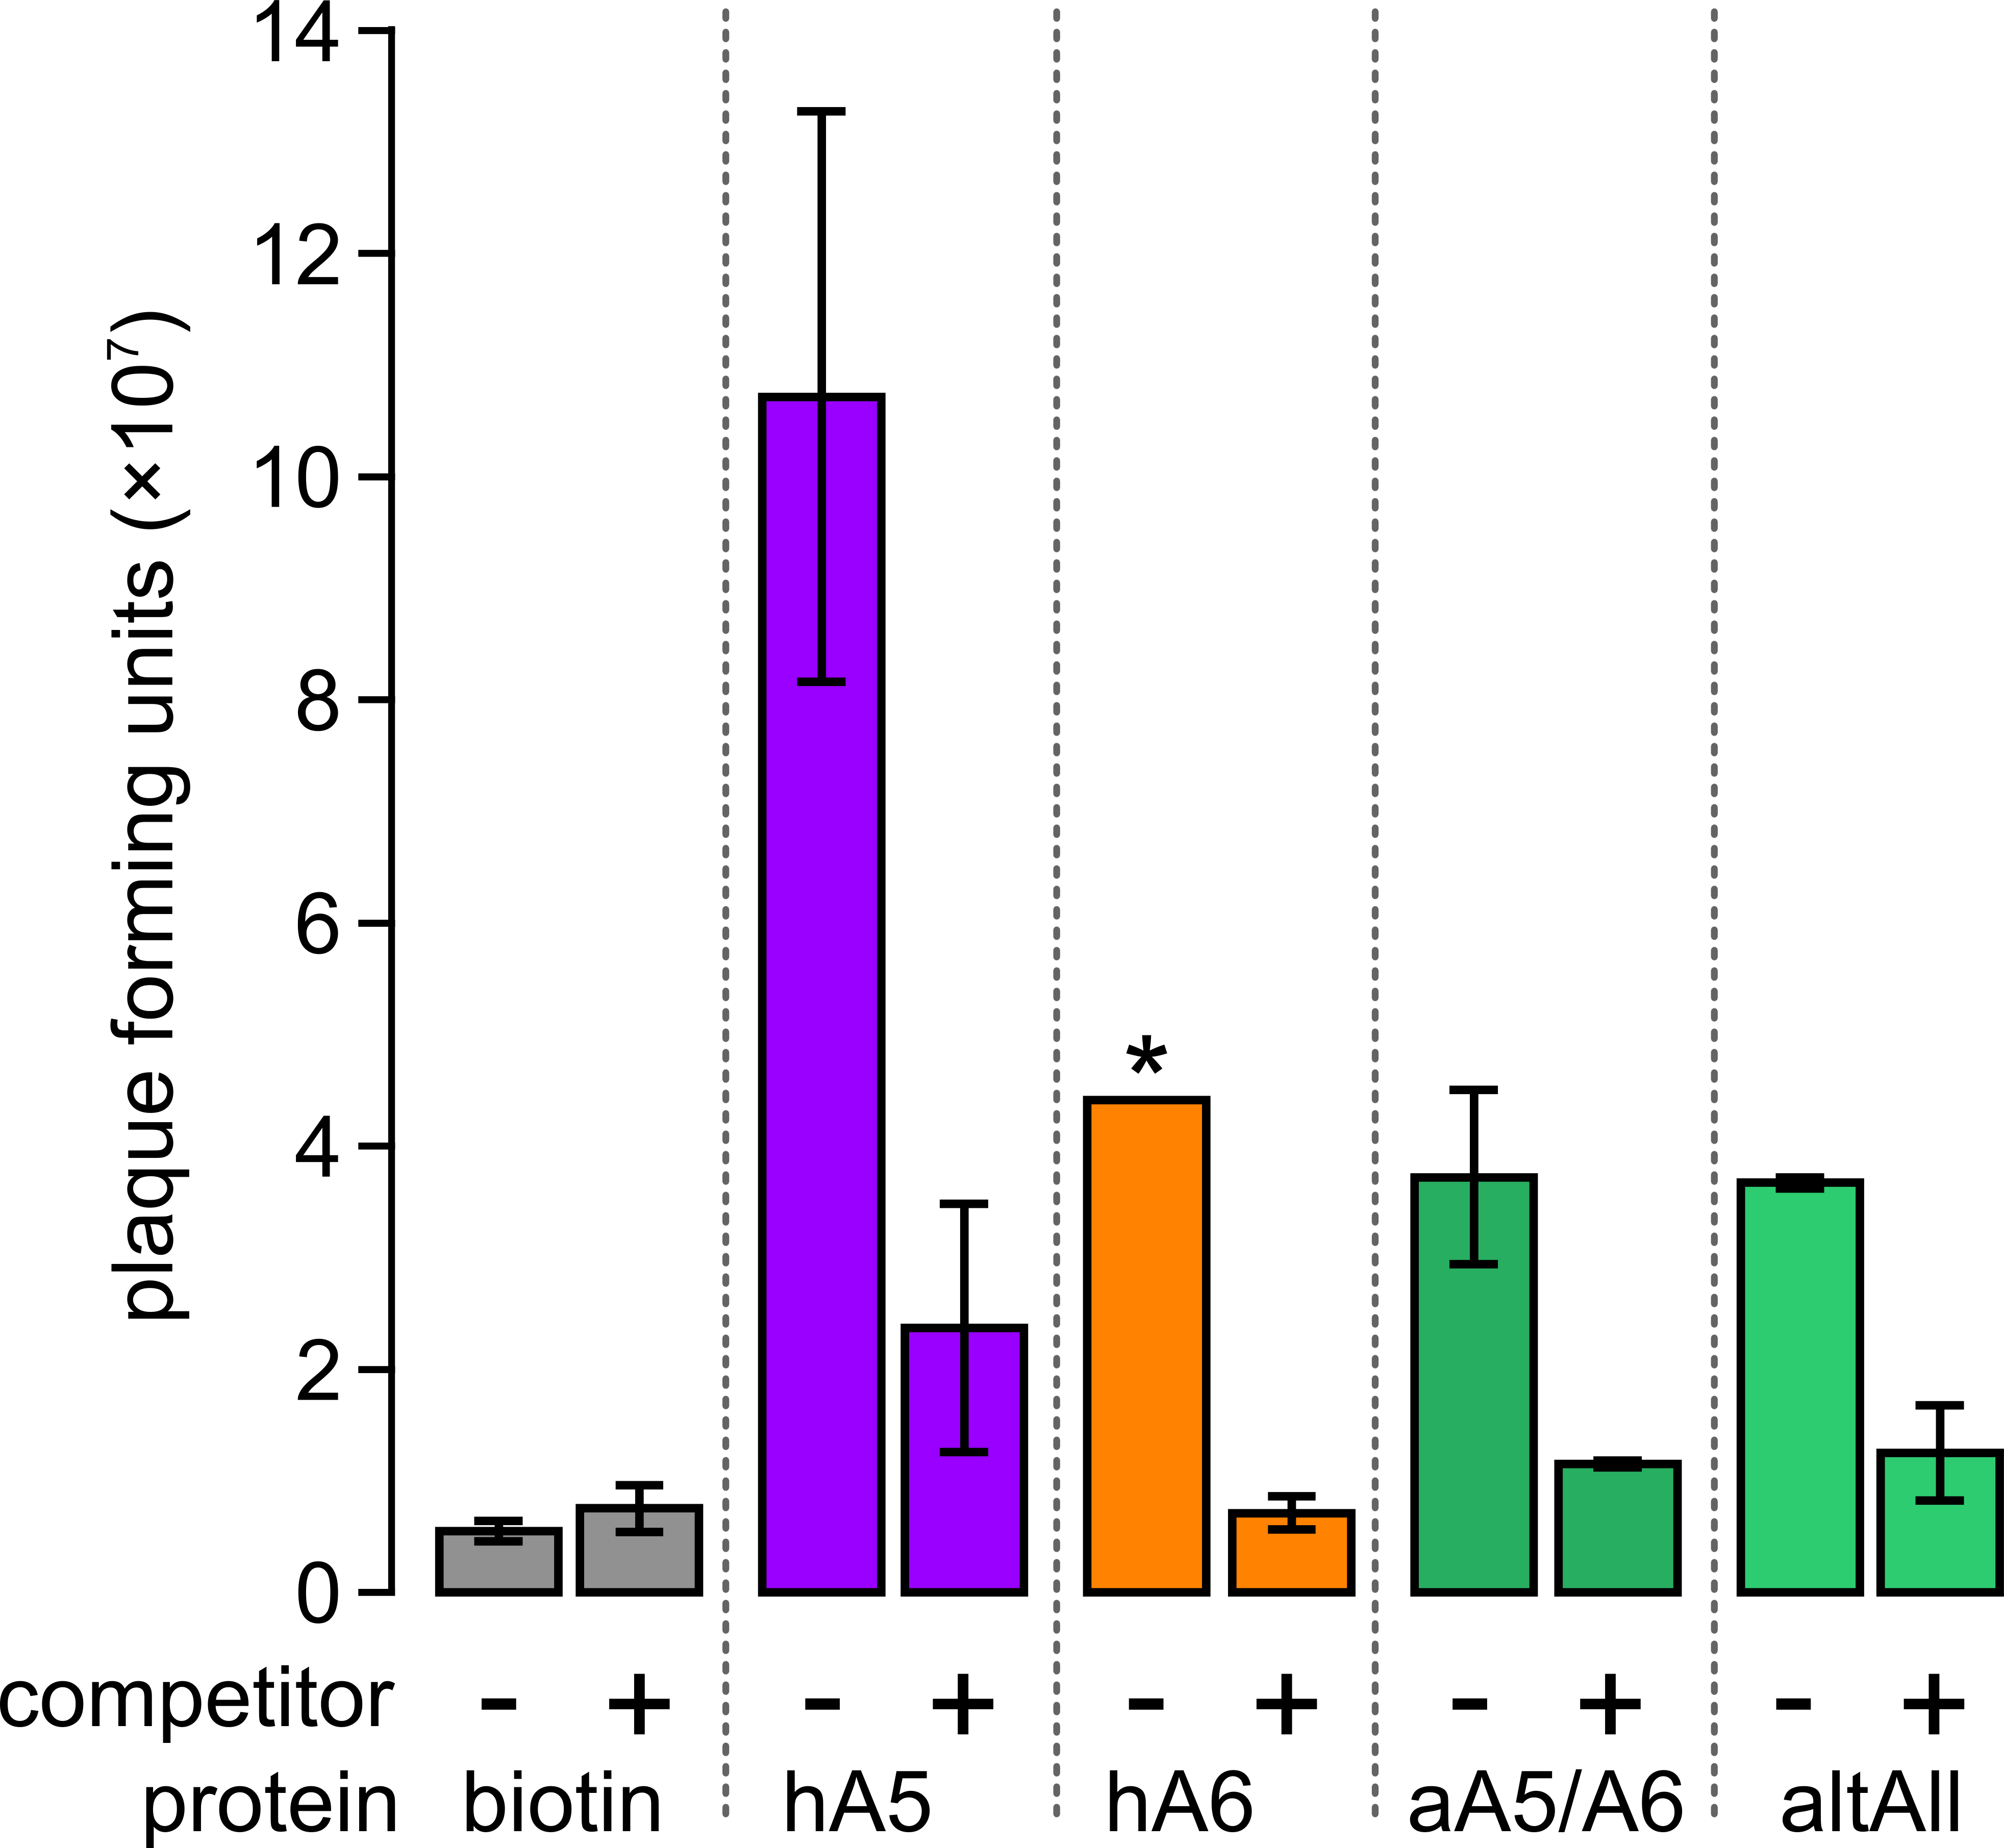
\includegraphics{ch6-figS1.png} 
\caption[Phage enrichment is reduced by the competitor
peptide]{Phage enrichment is reduced in the presence of competitor
peptide. Figure shows eluted plaque forming units (PFU) (estimated
from phage titer) for two biological replicates of each condition.
Enrichment is shown for biotin-only control (gray), hA5 (purple),
hA6 (orange), ancA5/A6 (dark green), and ancA5/A6 atlAll (light green)
with (+) and without (-) competitor peptide. Error bars show standard
error for two biological replicates. ({*}) hA6 without competitor
is shown for only one replicate due to failure of the titer for the
other replicate.\label{samplefigure}}	
\end{figure}

\begin{figure}%figure S2
\centering
	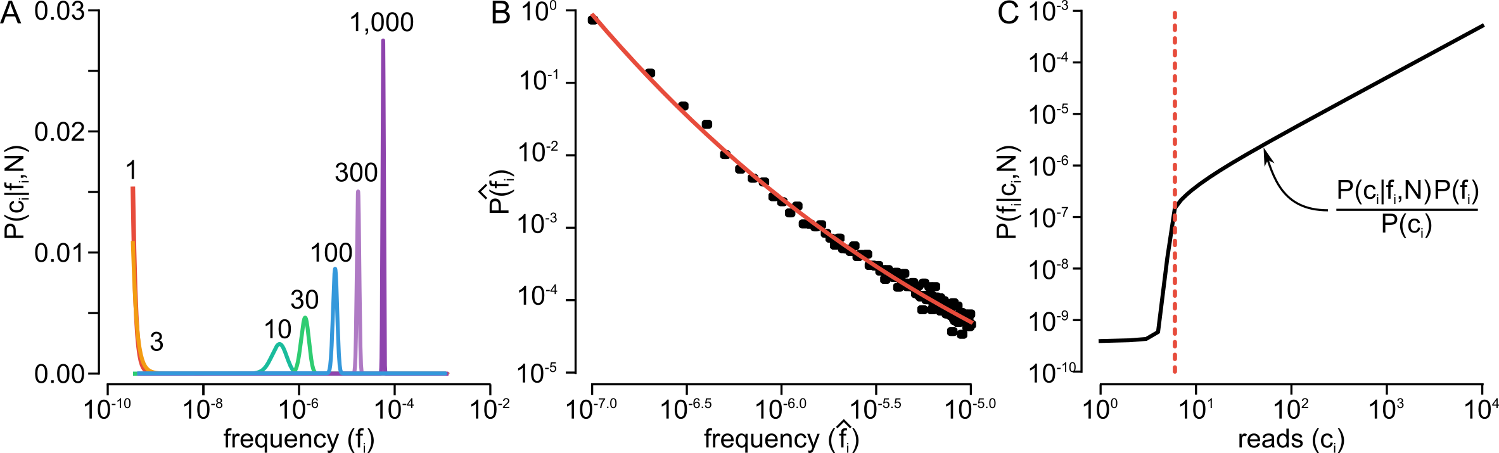
\includegraphics{ch6-figS2.png} 
\caption[We can identify the number of counts that reliably
reports on frequency in a sequenced phage pool]{We can identify the number of counts that reliably
reports on frequency in a sequenced phage pool. A) Using binomial
sampling, we can calculate the probability of observing exactly $c_{i}$
counts in $N$ samples from that has a peptide of actual frequency
$f_{i}$. Figure shows curves for counts ranging from 1 (red) to 1,000
(pink), all using $N=2.0\times10^{7}$. B) Panel shows a histogram
of frequencies estimated from 3.9$\times$$10^{7}$ reads taken from
the input library. The black points are experimental data. The red
curve is an exponential distribution fit to that curve. C) Using the
sampling from panel A and the fit curve from panel B, we can determine
$P(f_{i}|c_{i},N)$. The solid curve shows the relationship between
the number of reads for peptide $i$ (x-axis) against the maximum-likelihood
estimate of the frequency (y-axis). The red line highlights the cutoff
we used in our experiments.\label{samplefigure}}	
\end{figure}

\begin{figure}%figure S3
\centering
	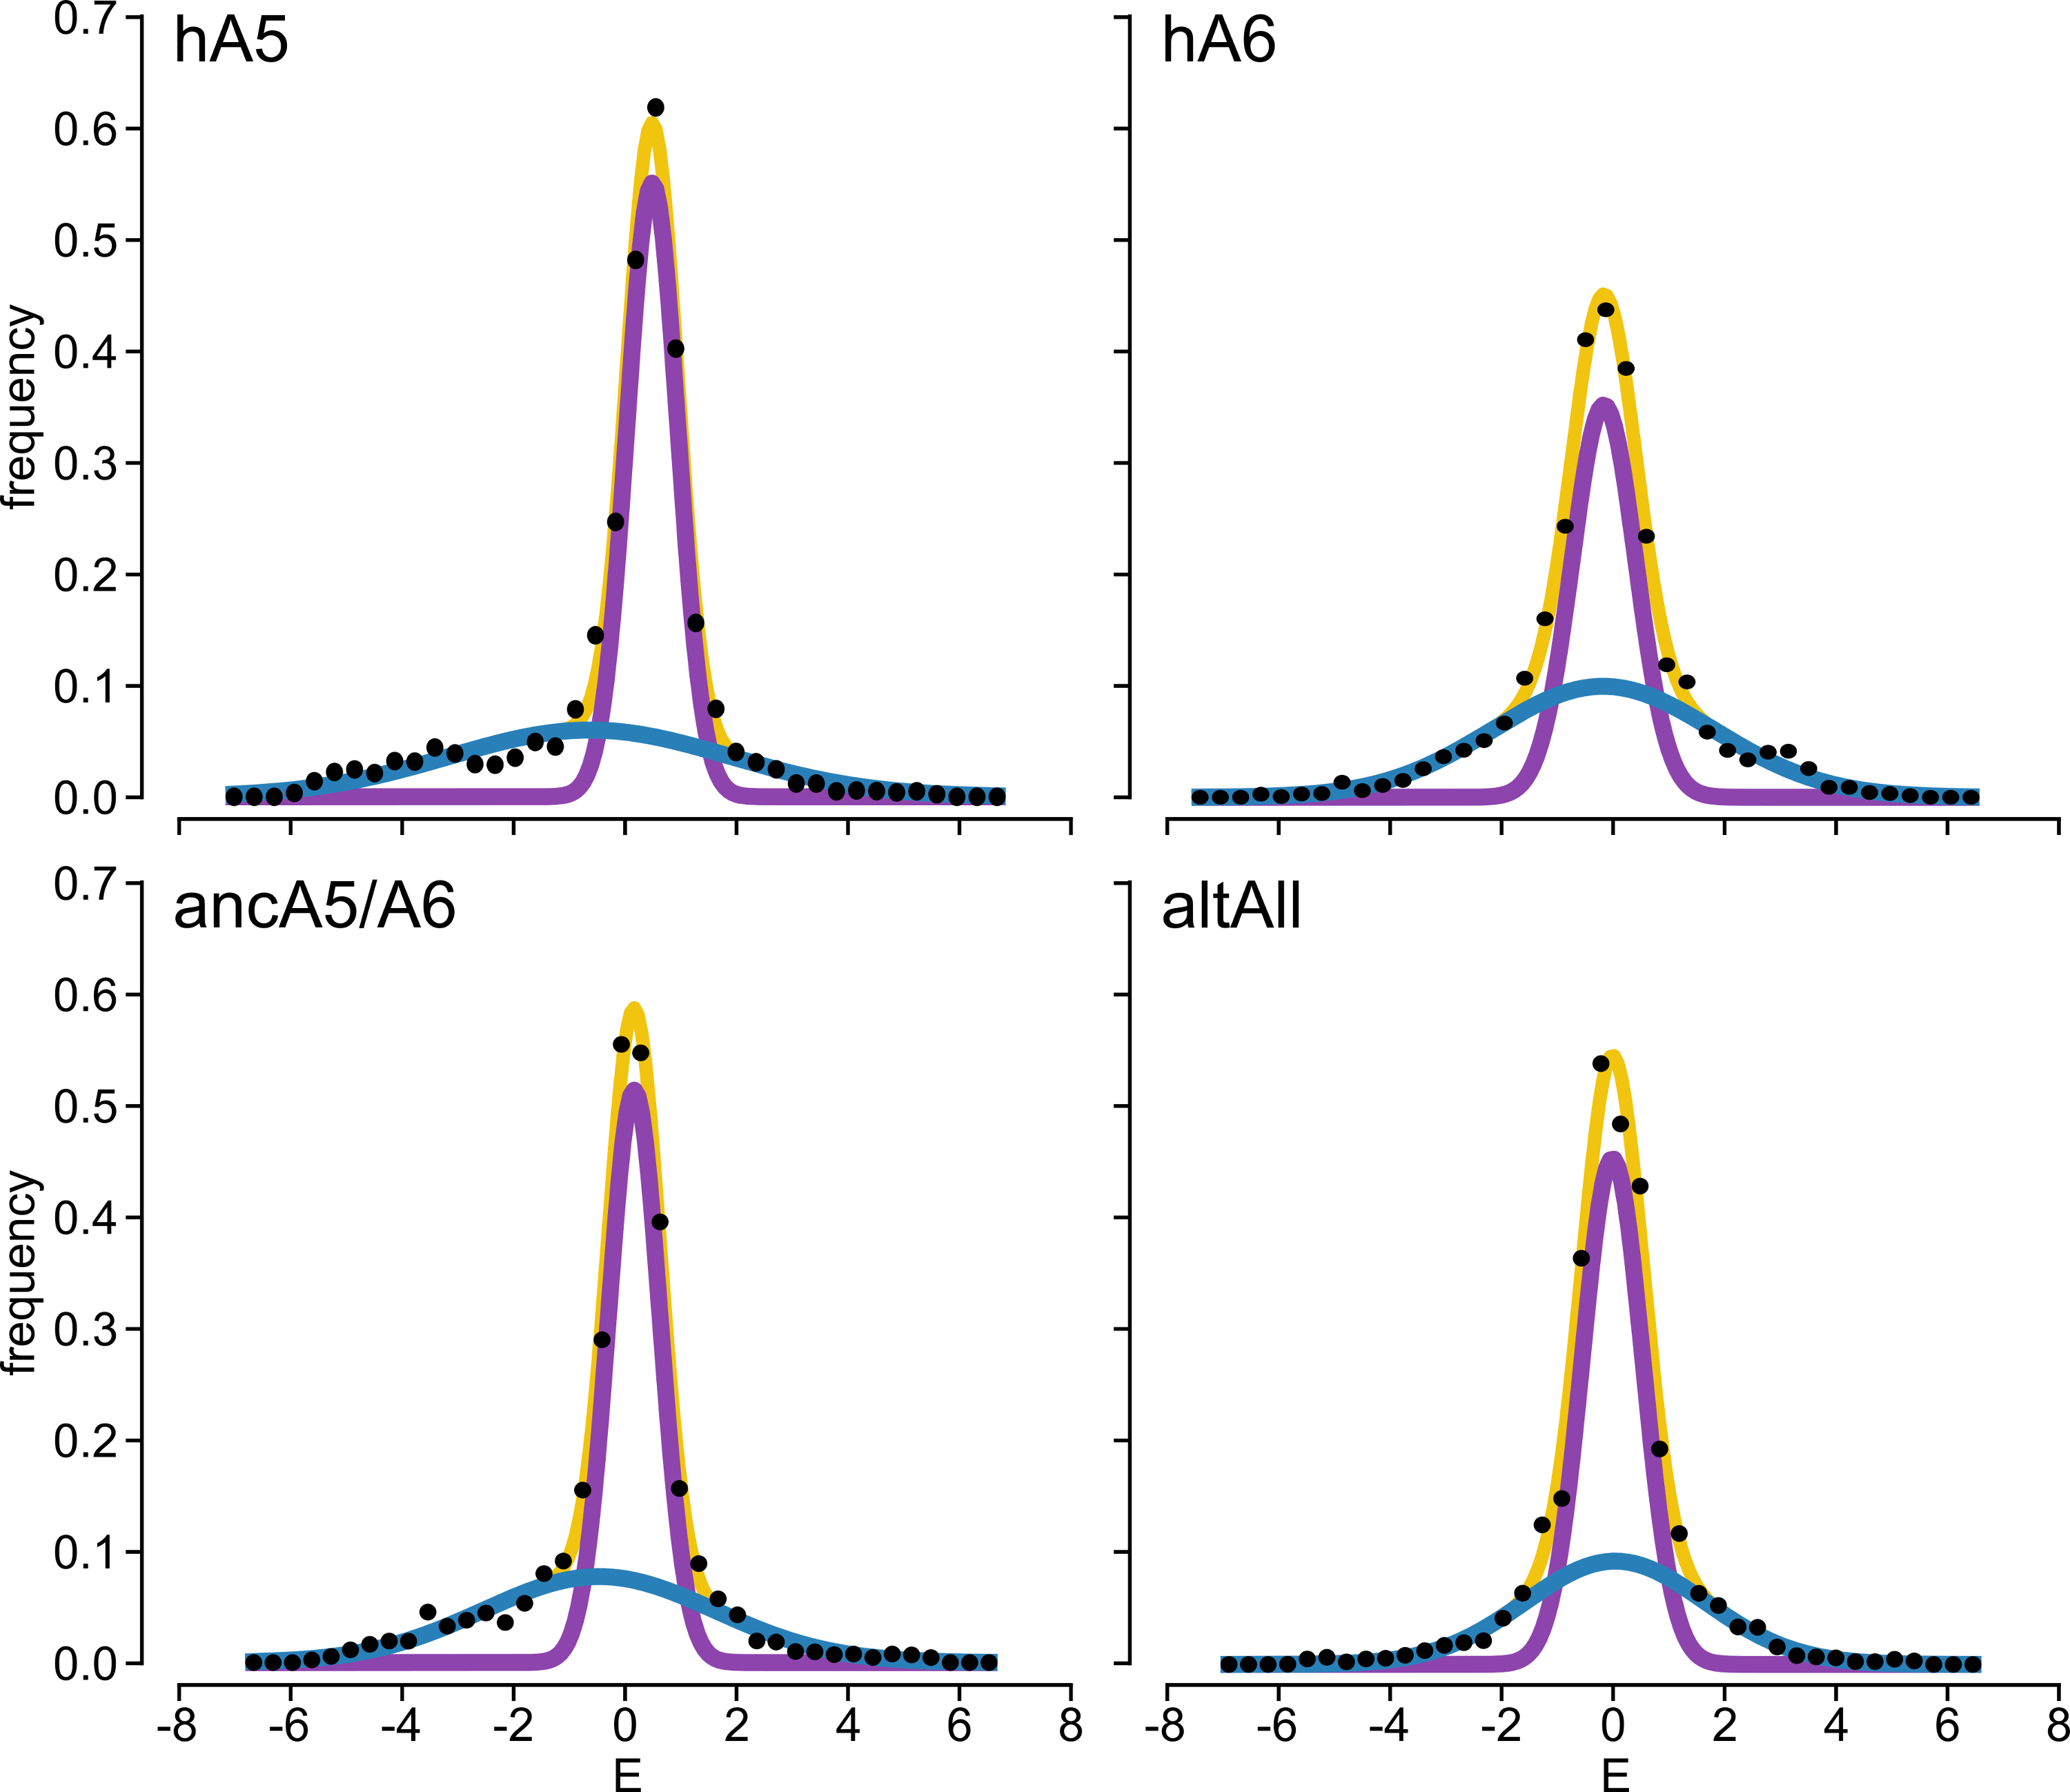
\includegraphics{ch6-figS3.png} 
\caption[Enrichment distributions for all proteins]{Enrichment distributions for all proteins. Panels show distribution of $E$ for
each protein (pooled bio-replicates). Points are raw histograms. Curves
are two Gaussian fit: blue (responsive), purple (unresponsive) and
yellow (sum).\label{samplefigure}}	
\end{figure}

\begin{figure}%figure S4
\centering
	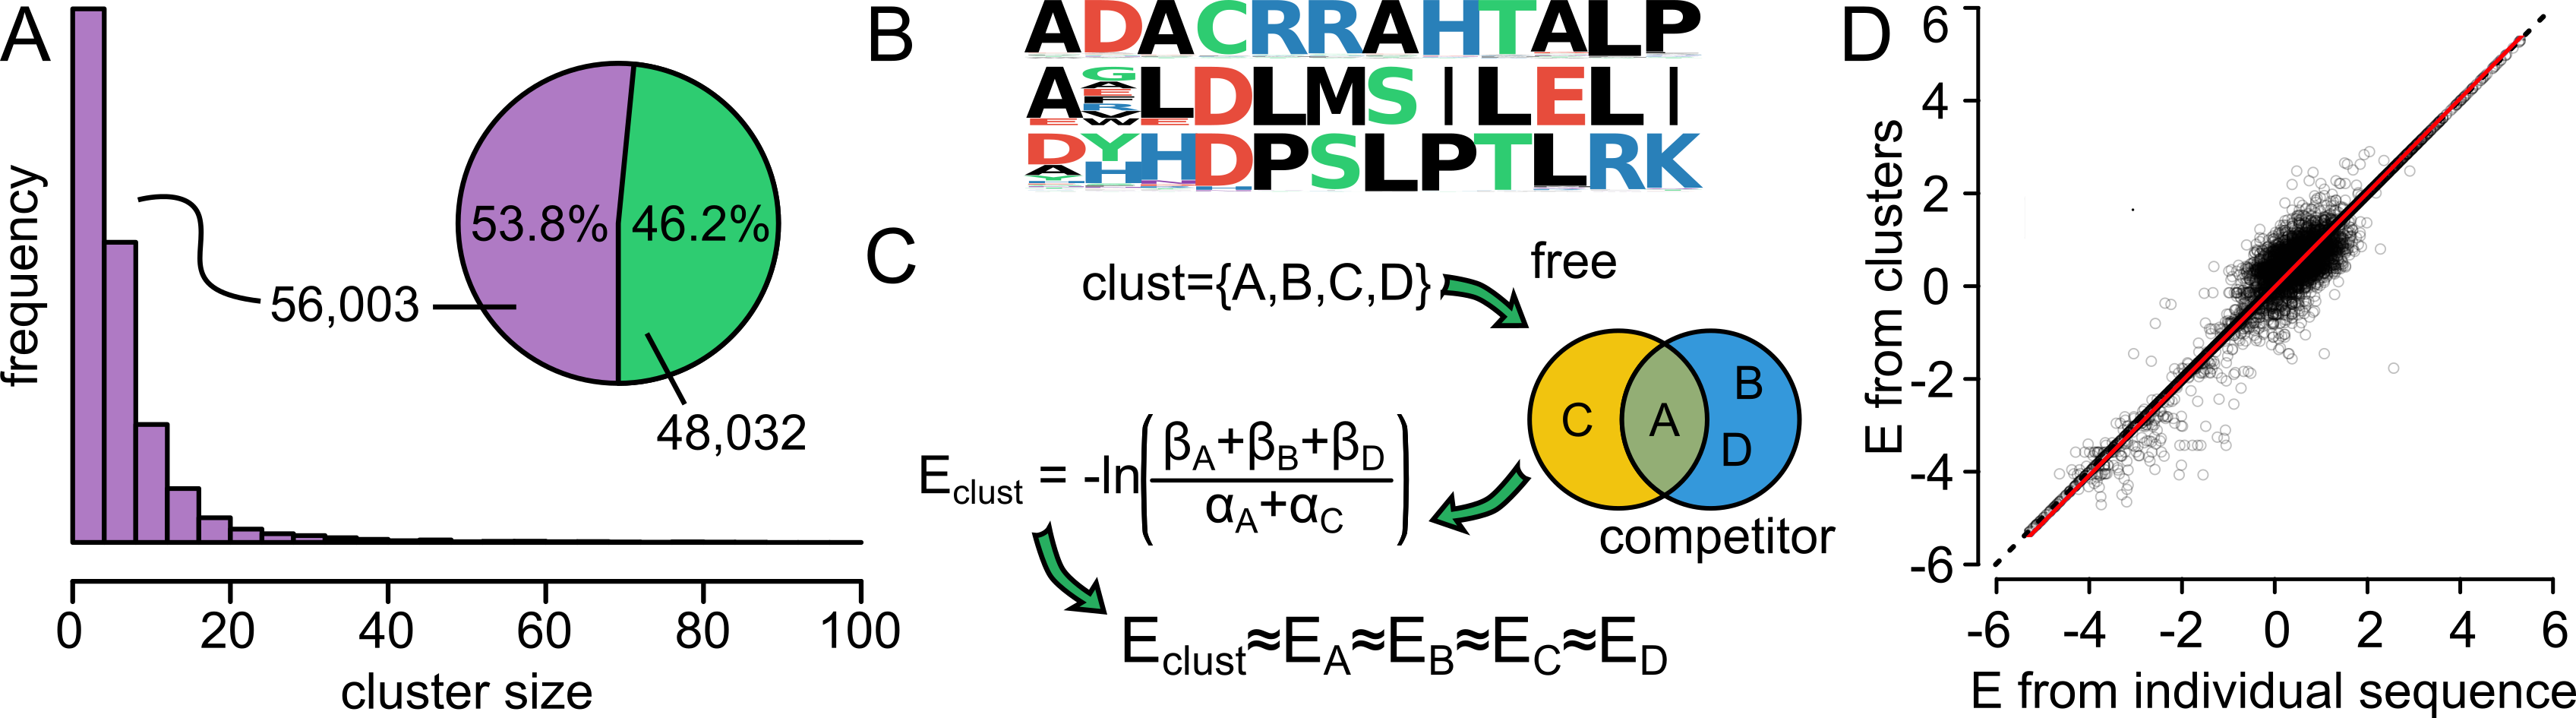
\includegraphics{ch6-figS4.png} 
\caption[We can estimate how addition of competitor 
alters frequencies]{We can estimate how addition of competitor peptide
alters the frequencies of peptides. A) Distribution of sizes of peptide
clusters from hA5 experiment. Pie chart shows number of peptides placed
in clusters (56,003; 53.8\%) versus not (48,032; 46.2\%). B) Three
example clusters taken from the clusters in panel A. The letter height
at each position indicates its frequency in the sequences within that
cluster. C) Toy example showing how enrichment is calculated for a
cluster containing peptides $\{A,B,C,D\}$. Peptides $A$ and $C$
were observed in the no competitor sample at frequencies $\alpha_{A}$
and $\alpha_{C}$. Peptides $A$, $B$, and $D$ were observed in
the competitor sample at frequencies $\beta_{A}$, $\beta_{B}$ and
$\beta_{D}$. The enrichment of the cluster is given by $E_{clust}=-ln[(\beta_{A}+\beta_{B}+\beta_{D})/(\alpha_{A}+\alpha_{C})]$.
All members of the cluster are then assigned E $\approx$ $E_{clust}$.
D) Comparison of enrichment values for hA5 peptides determined using
a direct comparison of frequencies with and without competitor (x-axis)
versus the clustering method (y-axis). Each point is an individual
peptide. Red line is a least-squares regression line fit to the data.
The dashed line is the 1:1 line.\label{samplefigure}}	
\end{figure}

\begin{figure}%figure S5
\centering
	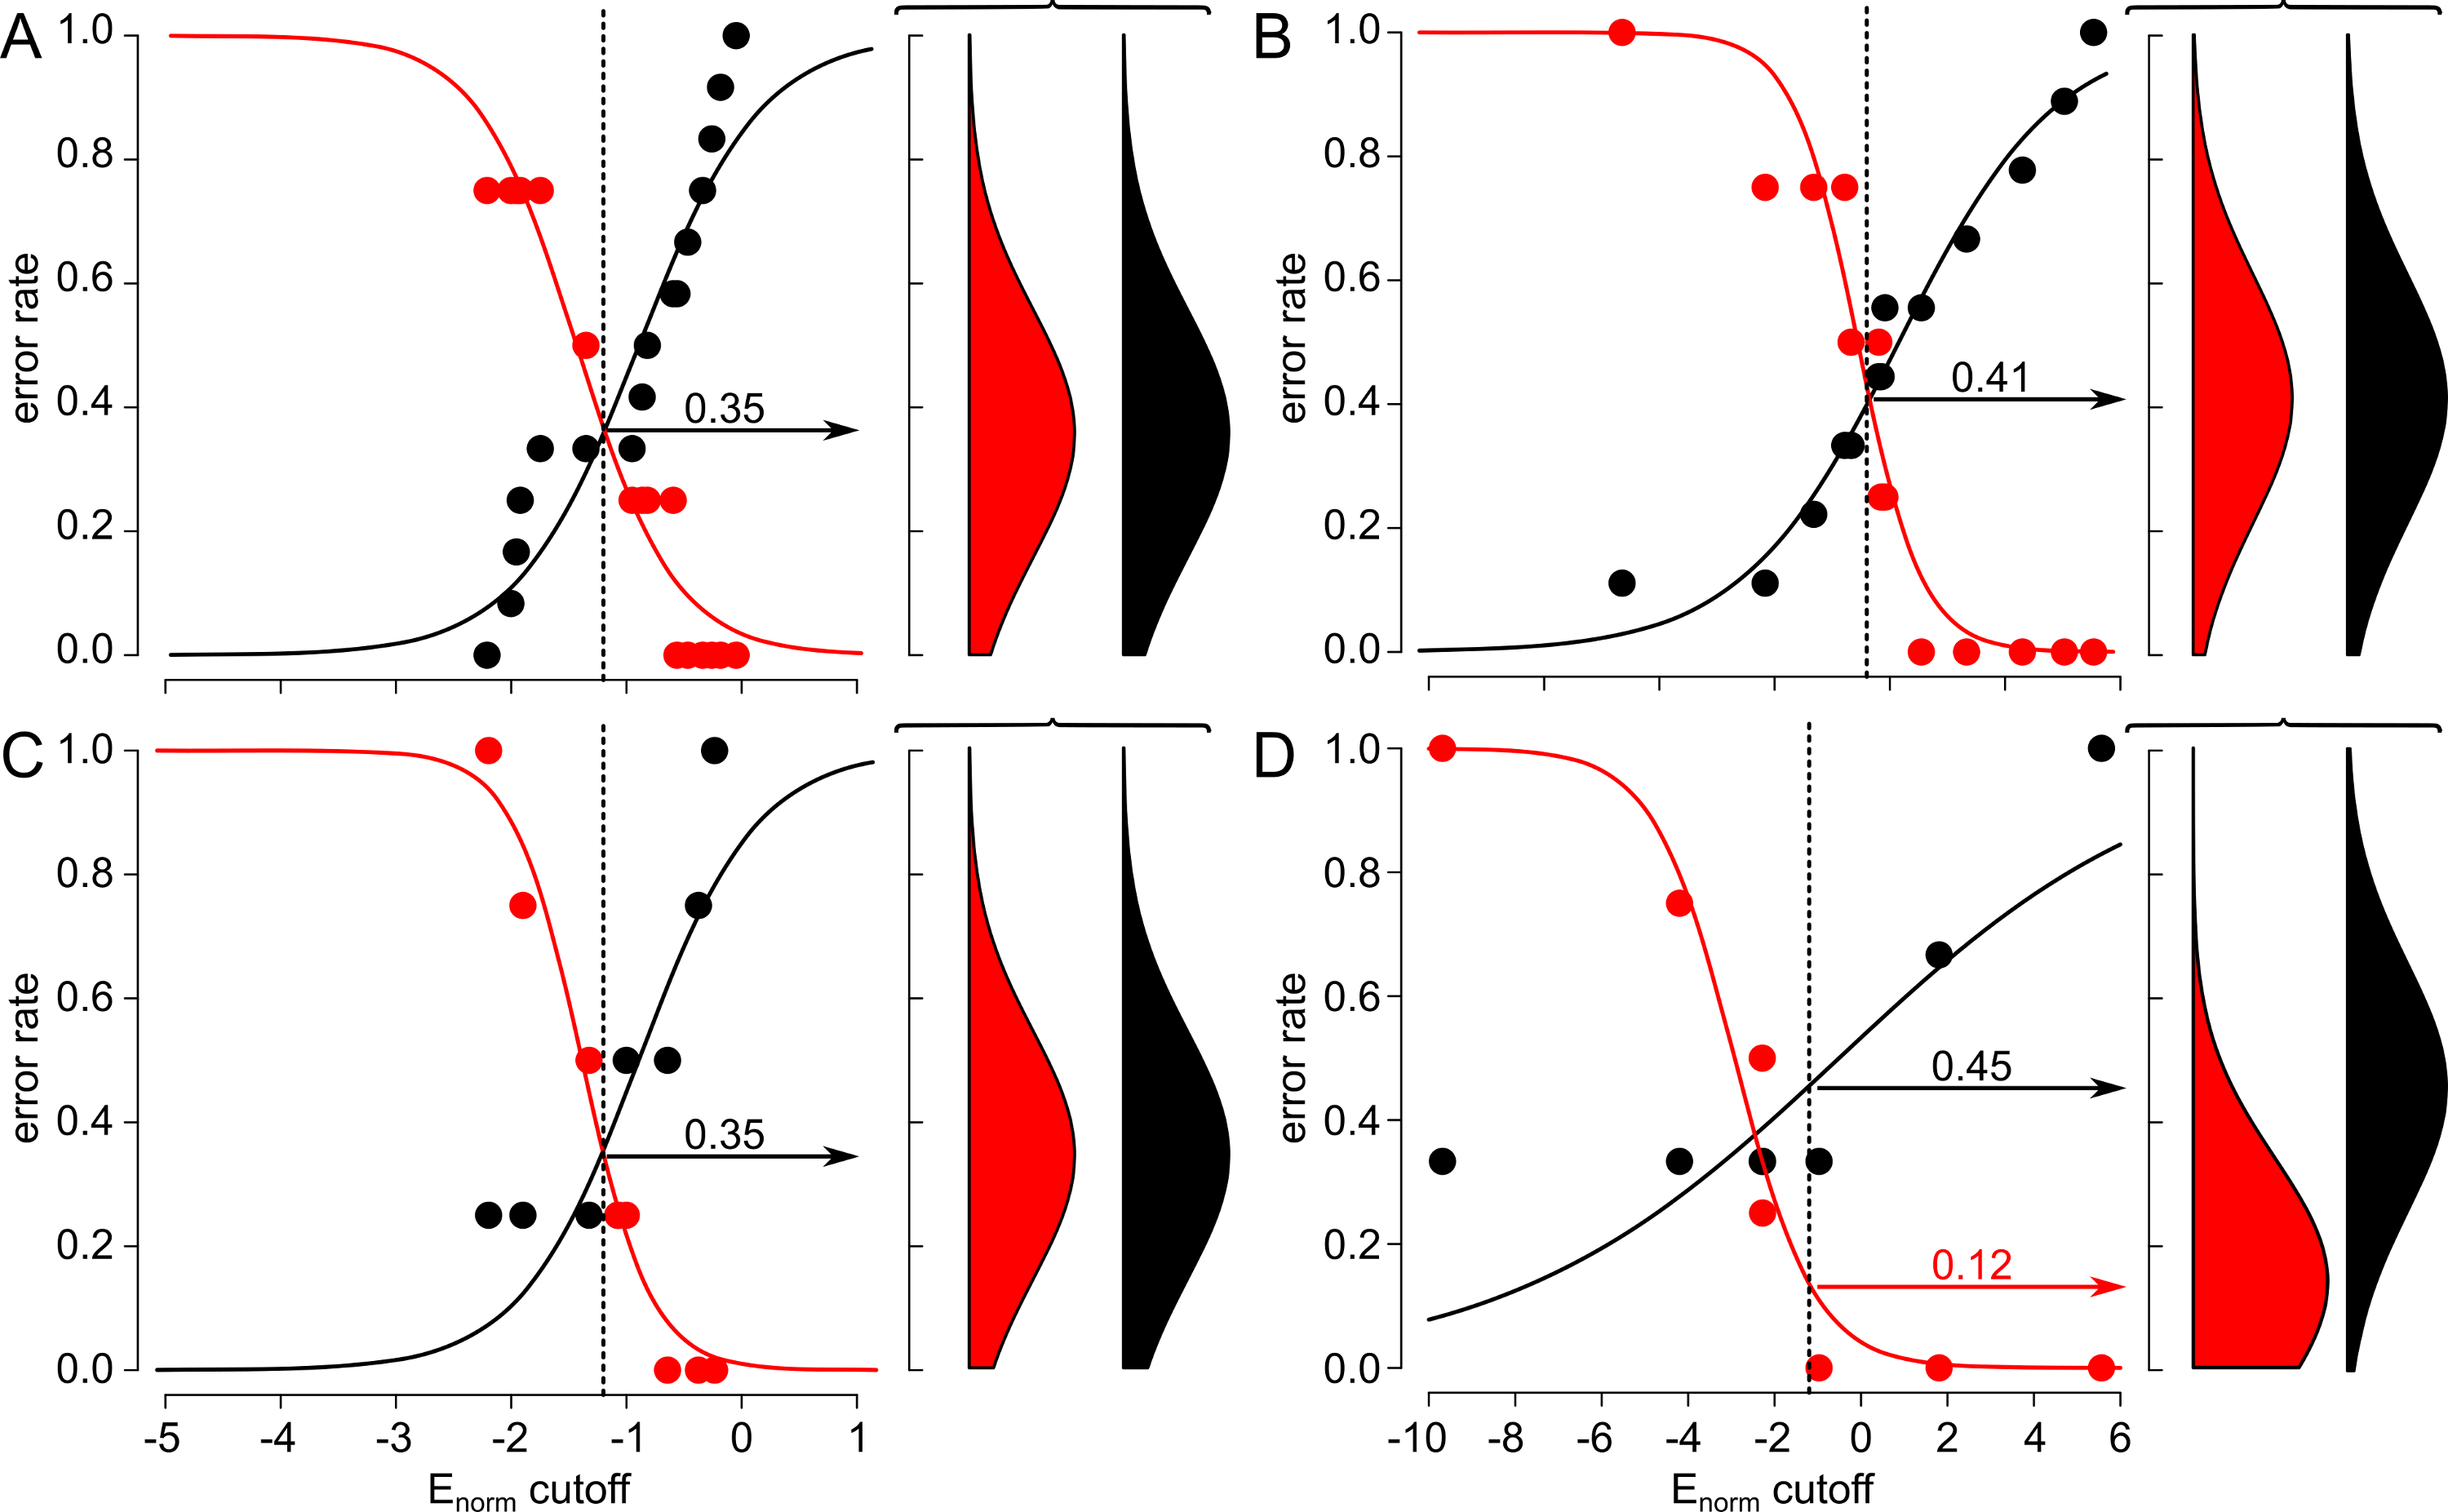
\includegraphics{ch6-figS5.png} 
\caption[Estimating the error rates for individual models]{Estimating the error rates for individual models. Panels show individual models: A) hA5, B) hA6, C) ancA5/A6, and D)
altAll. For each panel, the left graph shows the error rate for peptide
binding as a function of the cutoff in $E_{norm}$ chosen for classification.
Lines are fits of the modified Hill equation to the error rates. Colors
indicate the false negative rate (red) and false positive rate (black).
The dashed vertical line indicates the cutoff used for prediction
of the Venn diagrams in Fig 6 ($E_{norm}$ = -1.19). The error rates
associated with $E_{norm}$ = -1.19 are indicated with arrows pointing
right. The distributions in each panel show the prior distributions
used for the false negative (red) and false positive (black) error
rates in the Bayesian estimator. These distributions are centered
at the error rate estimate, with standard deviations of 0.2.\label{samplefigure}}	
\end{figure}


\begin{table}[h!]\footnotesize %Table S1
\center
\caption[Number of sequencing reads for each
sample] {Number of sequencing reads for each
sample. Sample, and whether or not competitor was added, are indicated
on the right. Columns show biological replicates 1 or 2. ``total''
columns indicate reads returned by the Illumina software pipeline. ``good''
columns indicate reads that passed our quality control and were used
to calculate enrichment values.}
\scriptsize
\begin{tabular}{cc|rr|rr}
 &  & \multicolumn{2}{c|}{rep1} & \multicolumn{2}{c}{rep2}\tabularnewline
sample & competitor & total & good & total & good\tabularnewline
\hline 
hA5 & - & 24,794,016 & 19,695,958 & 29,085,203 & 16,773,567\tabularnewline
hA5 & + & 15,053,706 & 11,523,991 & 17,631,137 & 13,612,463\tabularnewline
\hline 
hA6 & - & 22,728,393 & 17,722,779 & 7,769,003 & 5,972,295\tabularnewline
hA6 & + & 13,953,466 & 11,004,701 & 23,026,469 & 18,128,759\tabularnewline
\hline 
ancA5/A6 & - & 23,690,810 & 18,387,038 & 14,534,333 & 11,034,524\tabularnewline
ancA5/A6 & + & 19,441,043 & 15,053,276 & 18,030,887 & 14,217,877\tabularnewline
\hline 
altAll & - & 34,565,905 & 18,387,038 & 17,975,086 & 13,343,678\tabularnewline
altAll & + & 17,091,918 & 13,111,649 & 19,703,343 & 15,300,950\tabularnewline
\hline 
raw library &  & 39,700,991 & 32,190,368 & --- & ---\tabularnewline
\end{tabular}
\end{table}



\begin{table}[h!]\footnotesize %Table S2
\center
\scriptsize
\caption[Features used in for supervised machine
learning] {Features used in for supervised machine
learning. Features denoted (CIDER) were calculated using the CIDER
software package \citep{holehouse_cider:_2015}. Other features were
calculated using our own software package (HOPS: https://github.com/harmslab/hops).}
\scriptsize
\begin{tabular}{c|c}
feature & ref\tabularnewline
\hline 
num. hbond acceptors & ---\tabularnewline
num. hbond donors & ---\tabularnewline
$\kappa$ (CIDER) & \citep{holehouse_cider:_2015}\tabularnewline
$\Delta$ (CIDER) & \citep{holehouse_cider:_2015}\tabularnewline
$\Omega$ (CIDER) & \citep{holehouse_cider:_2015}\tabularnewline
FER (CIDER) & \citep{holehouse_cider:_2015}\tabularnewline
$\Sigma$ (CIDER) & \citep{holehouse_cider:_2015}\tabularnewline
dmax (CIDER) & \citep{holehouse_cider:_2015}\tabularnewline
$\Delta$max & \citep{holehouse_cider:_2015}\tabularnewline
NCPR & \citep{holehouse_cider:_2015}\tabularnewline
$F_{+}$(CIDER) & \citep{holehouse_cider:_2015}\tabularnewline
$F_{-}$(CIDER) & \citep{holehouse_cider:_2015}\tabularnewline
FCR (CIDER) & \citep{holehouse_cider:_2015}\tabularnewline
mean hydropathy (CIDER) & \citep{holehouse_cider:_2015}\tabularnewline
White Interface scale & \citep{hessa_recognition_2005}\tabularnewline
Engleman scale & \citep{engelman_identifying_1986}\tabularnewline
$\%$ buried in structures & \citep{schein_solubility_1990}\tabularnewline
Kyte/Doolittle scale & \citep{kyte_simple_1982}\tabularnewline
Octanol scale & \citep{wimley_experimentally_1996}\tabularnewline
Hopp-Woods scale & \citep{hopp_prediction_1981}\tabularnewline
Uversky scale & \citep{holehouse_cider:_2015}\tabularnewline
cumulative mean hydropathy & \citep{holehouse_cider:_2015}\tabularnewline
side chain accessible area & \citep{hubbard_naccess_1993}\tabularnewline
main chain accessible area & \citep{hubbard_naccess_1993}\tabularnewline
Chou-Fasman, $\beta$ & \citep{chou_empirical_1978}\tabularnewline
Chou-Fasman, $\alpha$ & \citep{chou_empirical_1978}\tabularnewline
Chou-Fasman, turn & \citep{chou_empirical_1978}\tabularnewline
fraction poly-proline II & \citep{holehouse_cider:_2015}\tabularnewline
predicted charge at pH 4 & ---\tabularnewline
predicted charge at pH 5 & ---\tabularnewline
predicted charge at pH 6 & ---\tabularnewline
predicted charge at pH 7 & ---\tabularnewline
predicted charge at pH 8 & ---\tabularnewline
predicted charge at pH 9 & ---\tabularnewline
num. positive amino acids & ---\tabularnewline
num. neutral amino acids & ---\tabularnewline
num. negative amino acids & ---\tabularnewline
net charge & ---\tabularnewline
isoelectric point & ---\tabularnewline
knob main chain, b & \citep{joo_amino_2014}\tabularnewline
socket main chain, x & \citep{joo_amino_2014}\tabularnewline
socket main chain, y & \citep{joo_amino_2014}\tabularnewline
socket main chain, h & \citep{joo_amino_2014}\tabularnewline
knob side chain, b & \citep{joo_amino_2014}\tabularnewline
socket side chain, x & \citep{joo_amino_2014}\tabularnewline
socket side chain, y & \citep{joo_amino_2014}\tabularnewline
socket side chain, h & \citep{joo_amino_2014}\tabularnewline
side chain volume & \citep{richards_areas_1977}\tabularnewline
molecular weight & ---\tabularnewline
aromatic & ---\tabularnewline
\end{tabular}
\end{table}



\begin{table}[h!]\footnotesize %Table S3
\caption[Predicted $E$ and
measured binding constants for peptides] {Predicted $E$ and
measured binding constants for peptides. Columns indicate calculated
$E$ and measured $K_{D}$ for the peptides indicated on the left.
For $K_{D}$, an entry of ``$>$ 100'' indicates that we performed
an ITC experiment, but that no binding was detectable better than
$\approx$100 $\mu M$. An entry of ``---'' indicates no experiment
was performed.}
\scriptsize
\begin{tabular}{ll|rr|rr|rr|rr}
 &  & \multicolumn{2}{c|}{hA5} & \multicolumn{2}{c|}{hA6} & \multicolumn{2}{c|}{aA5A6} & \multicolumn{2}{c}{altAll}\tabularnewline
name & sequence & $E$ & $K_{D}$ & $E$ & $K_{D}$ & $E$ & $K_{D}$ & \emph{$E$} & $K_{D}$\tabularnewline
\hline 
Q86UW7 & AGSSQRAPPAPTREGRRD & -4.03 & $>$100 & 0.26 & --- & -0.77 & --- & 0.41 & ---\tabularnewline
An1 & AMVSEFLKQAWFIE & -1.71 & $>$100 & -1.68 & 13 & -1.73 & --- & -0.37 & ---\tabularnewline
O75170 & DAPGAGAPPAPGKKEAPP & -3.94 & $>$100 & 0.50 & $>$100 & -0.74 & --- & 0.78 & $>$100\tabularnewline
p3 & DWSSWVYRDTQTGGSAE & -1.26 & $>$100 & -1.10 & $>$100 & -1.28 & --- & -0.11 & ---\tabularnewline
p1 & EPSPVSMNEGTFGGSAE & -0.27 & --- & -0.54 & 10 & -0.34 & $>$100 & -0.45 & ---\tabularnewline
Q13424 & GAGGERWQRVLLSLAEDT & -4.45 & 3 & -1.11 & --- & -1.98 & --- & -0.10 & ---\tabularnewline
B2RNZ0 & KEIKTAMWRLFVKIYFLQK & -3.53 & $>$100 & -2.72 & $>$100 & -2.38 & $>$100 & -1.36 & $>$100\tabularnewline
p6 & QPELTQGRVGINGGGSAE & -1.02 & $>$100 & 0.30 & --- & -0.79 & --- & -0.08 & ---\tabularnewline
NCX1 & RRLLFYKYVYKR & -1.20 & 18 & -1.33 & $>$100 & -1.40 & 30 & -0.59 & 47\tabularnewline
A6cons & RSHSGFDWRWGMEALTGGGSAE & -1.97 & 3 & -0.84 & 5 & -1.12 & 1 & -0.14 & 9\tabularnewline
A5cons & RSHSSSFQDWLLSRLPGGGSAE & -2.75 & 3 & -0.81 & $>$100 & -2.05 & 11 & -0.32 & 24\tabularnewline
Q14147 & SEDDRAGPAPPGASDGVD & -3.88 & $>$100 & 0.71 & $>$100 & -1.20 & --- & 0.47 & ---\tabularnewline
SIP & SEGLMNVLKKIYEDG & -0.60 & $>$100 & -1.05 & 26 & -0.64 & 77 & -0.32 & 42\tabularnewline
p4 & SIGASELHVYRSGGSAE & -0.76 & $>$100 & -0.21 & $>$100 & -0.18 & $>$100 & -0.40 & ---\tabularnewline
p7 & STTVRNGESPNCGGSAE & -0.45 & $>$100 & -0.84 & --- & -0.24 & --- & 0.16 & ---\tabularnewline
p5 & STVHEILSKLSEGY & -0.19 & $>$100 & -0.85 & $>$100 & -0.13 & --- & 0.07 & ---\tabularnewline
p2 & TAKYLPMRPGPLGGGSAE & -1.79 & $>$100 & 0.20 & $>$100 & -1.04 & $>$100 & 0.25 & $>$100\tabularnewline
\end{tabular}
\end{table}
